\documentclass{amsart}
\usepackage{xcolor,tikz}
\usetikzlibrary[positioning]

\begin{document}

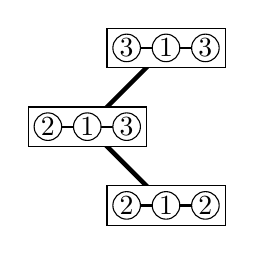
\begin{tikzpicture}[baseline=0cm, scale=0.5]
% top square 
\draw[style=ultra thick] (-5,0)--(-7,-2)--(-5,-4);

% left square
\draw[fill=white] (-6.5,-.5) rectangle (-3.5,.5);
\draw[style=thick](-6,0)--(-4,0);
\draw[radius=.35,fill=white](-6,0)circle node{3};
\draw[radius=.35,fill=white](-5,0)circle node{1};
\draw[radius=.35,fill=white](-4,0)circle node{3};

\draw[fill=white] (-8.5,-2.5) rectangle (-5.5,-1.5);
\draw[style=thick](-8, -2)--(-6,-2);
\draw[radius=.35,fill=white](-8,-2)circle node{2};
\draw[radius=.35,fill=white](-7,-2)circle node{1};
\draw[radius=.35,fill=white](-6,-2)circle node{3};


\draw[fill=white] (-6.5,-4.5) rectangle (-3.5,-3.5);
\draw[style=thick](-6,-4)--(-4,-4);
\draw[radius=.35,fill=white](-6,-4)circle node{2};
\draw[radius=.35,fill=white](-5,-4)circle node{1};
\draw[radius=.35,fill=white](-4,-4)circle node{2}; 
\end{tikzpicture}

\end{document}